\subsection{Conservation Laws}
\subsubsection{Conservation of Mass} Consider a small test volume $V$
with surface $A$. The rate of change of the mass in the volume is
\begin{equation}\label{mass:rate}
    \frac{d}{dt}\int_V\rho\,dV =
    \int_V\frac{\partial\rho}{\partial t}\,dV
\end{equation}
The derivative can be moved inside the integral because the test
volume is fixed in position.

The mass flow out of the surface is given by
\begin{equation}
    \int_A\rho\mathbf{u}\cdot\mathbf{n}\,dA =
    \int_V\nabla\cdot(\rho\mathbf{u})\,dV
\end{equation}
where divergence theorem was used to change the equation into a
volume integral.
\newslide
From the law of conservation of mass, the rate of change of the mass
in the volume must be equal to the mass flow \emph{into} the
surface, thus
\begin{align}
    &\int_V\frac{\partial\rho}{\partial t}\,dV =
    -\int_V\nabla\cdot(\rho\mathbf{u})\,dV\notag\\
    &\int_V\Bigl[(\frac{\partial\rho}{\partial t}+\nabla\cdot(\rho\mathbf{u})\Bigr]\,dV = 0\label{mass:con}
\end{align}
Since the test volume is arbitrary, the function inside the bracket
[ ] must vanish everywhere. Hence
\begin{equation}\label{mass:cont}
\boxed{\frac{\partial\rho}{\partial t}+\nabla\cdot(\rho\mathbf{u}) =
0}
\end{equation}
\newslide
It can be written in material derivative:
\begin{equation}\label{mass:cont2}
\frac{D\rho}{Dt}+\rho\nabla\cdot\mathbf{u} = 0
\end{equation}
For an incompressible fluid, $D\rho/Dt=0$, the equation of
continuity is reduced to
\begin{equation}\label{mass:cont3}
\nabla\cdot\mathbf{u} = 0
\end{equation}
\newslide
\subsubsection{Conservation of Momentum} From the law of conservation
of momentum, consider a same fixed volume $V$:
\begin{equation}\label{mom:con}
    \frac{d}{dt}(\text{momentum in }V)= - \text{momentum leakage} +
    \sum(\text{applied force})
\end{equation}
The rate of change of mometum in the volume is
\begin{equation}\label{mom:rate}
    \frac{d}{dt}\int_V\rho u_i\,dV =
    \int_V\frac{\partial\rho u_i}{\partial t}\,dV
\end{equation}
where $u_i$ is the $i$th component of the velocity $\mathbf{u}$.
Similar to \eqref{mass:rate}, the derivative can be moved inside the
integral.
\newslide
The momentum leakage (in component form) is given by
\begin{equation}\label{mom:leakage}
    \int_A(\rho u_i)u_j(n_j\,dAj) =
    \int_V\frac{\partial}{\partial x_j}(\rho u_i u_j)\,dV
\end{equation}
where divergence theorem was applied again.

The applied forces consist of body force and surface force.
\newslide
The body force is simply
\begin{equation}\label{mom:bodyf}
    \text{body force} = \int_V\rho f_i\,dV
\end{equation}
where $f_i$ is the component of the body force per unit mass.
\newslide
Considered a tetrahedral volume of fluid.
\begin{figure}[htpb]
  \centering
  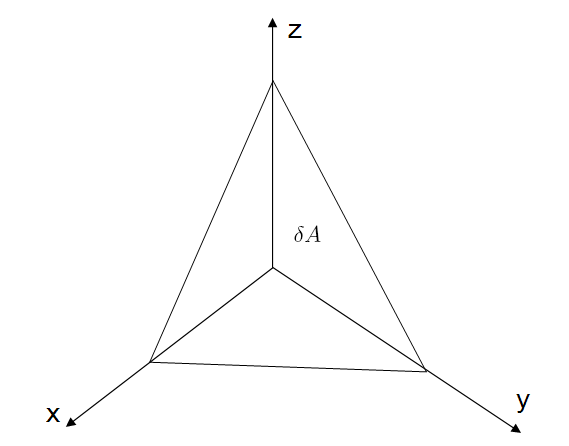
\includegraphics[width=0.9\textheight]{stress.png}\\
  \caption{Stress on a tetrahedral volume of fluid}\label{stress}
\end{figure}
\newslide
The sum of the surface force must be zero by Newton's second
law\footnote{Otherwise it will be accelerating.}. The area of the
``big triangle'' is given by $\delta A$, while the area of other
three surfaces are given by
\begin{subequations}
\begin{align}
    \delta A_1&=\mathbf{a}\cdot \mathbf{n} \delta A\\
    \delta A_2&=\mathbf{b}\cdot \mathbf{n} \delta A\\
    \delta A_3&=\mathbf{c}\cdot \mathbf{n} \delta A
\end{align}
\end{subequations}

\newslide
The sum of surface force is
\begin{align}
    \Sigma_i(\mathbf{n})\delta A + \Sigma_i(-\mathbf{a})\delta A_1 + \Sigma_i(-\mathbf{b})\delta
    A_2 + \Sigma_i(-\mathbf{c})\delta A_3 = 0\notag\\
    \Sigma_i(\mathbf{n})\delta A - \Sigma_i(\mathbf{a})\mathbf{a}\cdot \mathbf{n}\delta A
     - \Sigma_i(\mathbf{b})\mathbf{b}\cdot \mathbf{n}\delta
    A - \Sigma_i(\mathbf{c})\mathbf{c}\cdot \mathbf{n}\delta A = 0
\end{align}
Since $\Sigma$ is an odd function by Newton's third law. Then
\begin{equation}\label{mom:surf1}
    \Sigma_i(\mathbf{n}) = [ a_j\Sigma_i(\mathbf{a}) + b_j\Sigma_i(\mathbf{b}) +
    c_j\Sigma_i(\mathbf{c})] n_j
\end{equation}
Define the stress vector as
\begin{equation}\label{mom:surf1}
    \sigma_{ij} = a_j\Sigma_i(\mathbf{a}) + b_j\Sigma_i(\mathbf{b}) +
    c_j\Sigma_i(\mathbf{c})
\end{equation}
The total force on a surface is
\begin{equation}\label{mom:surf}
    \text{surface force} = \int_A\sigma_{ij}n_j\,dA = \int_V\frac{\partial}{\partial x_j}\sigma_{ij}\,dV
\end{equation}
\newslide
Combining \eqref{mom:rate}, \eqref{mom:leakage}, \eqref{mom:bodyf}
and \eqref{mom:surf}, \eqref{mom:con} can be written as:
\begin{equation}\label{mom:con2}
    \int_V\frac{\partial\rho u_i}{\partial t}\,dV = - \int_V\frac{\partial}{\partial x_j}(\rho u_i
    u_j)\,dV + \int_V\rho f_i\,dV + \int_V\frac{\partial}{\partial x_j}\sigma_{ij}\,dV
\end{equation}
Since the test volume is arbitrary, the integrands can be taken out
from the integrals:
\begin{equation}\label{mom:con3}
    \frac{\partial\rho u_i}{\partial t} + \frac{\partial}{\partial x_j}(\rho u_i
    u_j) = \rho f_i + \frac{\partial}{\partial x_j}\sigma_{ij}
\end{equation}
Applying the equation of continuity \eqref{mass:cont} in component
form,
\begin{equation*}
\frac{\partial\rho}{\partial t}+\frac{\partial}{\partial x_j}(\rho
u_j) = 0
\end{equation*}
\newslide
The left side of \eqref{mom:con3} can be further simplified:
\begin{align*}
    \frac{\partial\rho u_i}{\partial t} + \frac{\partial}{\partial x_j}(\rho u_i
    u_j) &= \rho\frac{\partial u_i}{\partial t} + u_i\frac{\partial\rho}{\partial t} +
    u_i\frac{\partial}{\partial x_j}(\rho u_j) + \rho u_j\frac{\partial}{\partial
    x_j}(u_i)\\
    &= \rho\frac{\partial u_i}{\partial t} + u_i\Bigl[\frac{\partial\rho}{\partial t} +
    \frac{\partial}{\partial x_j}(\rho u_j)\Bigr] + \rho u_j\frac{\partial}{\partial
    x_j}(u_i)\\
    &= \rho\frac{\partial u_i}{\partial t} + \rho u_j\frac{\partial}{\partial
    x_j}(u_i)\\
    &= \rho\frac{D u_i}{D t}
\end{align*}
\newslide
The momentum equation is
\begin{equation}\label{mom:eq}
    \boxed{\rho\frac{D u_i}{D t} = \rho f_i + \frac{\partial}{\partial
    x_j}\sigma_{ij}}
\end{equation}

Navier-Stokes equation will be derived from the conservation of
momentum equation.
